%\RequirePackage[l2tabu, orthodox]{nag}
\RequirePackage{currfile}
\documentclass[12pt]{beamer}
\graphicspath{{Imagenes/}{../Imagenes/}}
\usepackage[utf8]{inputenc}
\usepackage[spanish]{babel}
\usepackage{standalone}
\usepackage{color}
\usepackage[binary-units=true]{siunitx}
\usepackage{hyperref}
\hypersetup{
  colorlinks=true,
  linkcolor=blue,          % color of internal links (change box color with linkbordercolor)
  citecolor=green,        % color of links to bibliography
  filecolor=magenta,      % color of file links
  urlcolor=cyan,           % color of external links
  linkbordercolor={0 0 1}
}
\usepackage{xcolor, soul}
\usepackage{etoolbox}
\usepackage{amsmath}
\usepackage{amsthm}
\usepackage{physics}
\usepackage{multicol}
\usepackage{graphicx}
\usepackage{bookmark}
\usepackage{longtable}
\usepackage{graphicx}
\usepackage{tikz}
\usepackage[siunitx, RPvoltages]{circuitikz}
\usetikzlibrary{mindmap}
\usetikzlibrary{arrows, patterns, shapes, decorations.markings, decorations.pathmorphing}
\usetikzlibrary{matrix,positioning}
\tikzstyle{every picture}+=[remember picture,baseline]
\usepackage[autostyle,spanish=mexican]{csquotes}
\usepackage{pifont}
\usepackage[font=footnotesize,textfont=it]{caption}
\usepackage{tabulary}
\usepackage{booktabs}
\usepackage[outdir=./]{epstopdf}
%\usepackage{epstopdf}
\usepackage{media9}
\usepackage{multimedia}
\usepackage{bigints}
%\usepackage{enumitem}
\usepackage[os=win]{menukeys}
\usepackage{pifont}
\usepackage{pbox}
\usepackage{alltt}
\usepackage{verbatim}
\usepackage{colortbl}
\usepackage{tcolorbox}
\usepackage{fancyvrb}
\usepackage[sfdefault]{roboto}  %% Option 'sfdefault' only if the base font of the document is to be sans serif
%\usepackage[T1]{fontenc}
\setcounter{secnumdepth}{3}
\setcounter{tocdepth}{3}
\DeclareGraphicsExtensions{.pdf,.png,.jpg}
\renewcommand {\arraystretch}{1.5}
\definecolor{ao}{rgb}{0.0, 0.5, 0.0}
\definecolor{aquamarine}{rgb}{0.5, 1.0, 0.83}
\definecolor{kellygreen}{rgb}{0.3, 0.73, 0.09}
\definecolor{bisque}{rgb}{1.0, 0.89, 0.77}
\definecolor{amber}{rgb}{1.0, 0.75, 0.0}
\definecolor{armygreen}{rgb}{0.29, 0.33, 0.13}
\definecolor{alizarin}{rgb}{0.82, 0.1, 0.26}
\definecolor{cadetblue}{rgb}{0.37, 0.62, 0.63}
\newcommand*{\TitleParbox}[1]{\parbox[c]{6cm}{\raggedright #1}}%
\newcommand{\python}{\texttt{python}}
\newcommand{\textoazul}[1]{\textcolor{blue}{#1}}
\newcommand{\azulfuerte}[1]{\textcolor{blue}{\textbf{#1}}}
\newcommand{\funcionazul}[1]{\textcolor{blue}{\textbf{\texttt{#1}}}}
%\normalfont
\usepackage{ccfonts}% http://ctan.org/pkg/{ccfonts}
\usepackage[T1]{fontenc}% http://ctan.or/pkg/fontenc
\renewcommand{\rmdefault}{cmr}% cmr = Computer Modern Roman
\usefonttheme[onlymath]{serif}
\linespread{1.3}
\newcounter{saveenumi}
\newcommand{\seti}{\setcounter{saveenumi}{\value{enumi}}}
\newcommand{\conti}{\setcounter{enumi}{\value{saveenumi}}}
\newcommand{\tikzmark}[1]{\tikz[remember picture] \node[coordinate] (#1) {#1};}

\usepackage{scalerel}[2016-12-29]
\def\stretchint#1{\vcenter{\hbox{\stretchto[440]{\displaystyle\int}{#1}}}}
\def\scaleint#1{\vcenter{\hbox{\scaleto[3ex]{\displaystyle\int}{#1}}}}
\def\bs{\mkern-12mu}

\newtheorem{teo}{}[section]
\usepackage{blkarray}

%reduce el tamaño de letra de la etiqueta equations
\makeatletter
\def\maketag@@@#1{\hbox{\m@th\normalfont\small#1}}
\makeatother

%se usa para la x en itemize
\newcommand{\xmark}{\text{\ding{55}}}

%\AtBeginDocument{\setlength{\tymin}{1em}}


\definecolor{myblue}{rgb}{.8, .8, 1}

\usepackage{empheq}

\newlength\mytemplen
\newsavebox\mytempbox

\makeatletter
\newcommand\mybluebox{%
    \@ifnextchar[%]
       {\@mybluebox}%
       {\@mybluebox[0pt]}}

\def\@mybluebox[#1]{%
    \@ifnextchar[%]
       {\@@mybluebox[#1]}%
       {\@@mybluebox[#1][0pt]}}

\def\@@mybluebox[#1][#2]#3{
    \sbox\mytempbox{#3}%
    \mytemplen\ht\mytempbox
    \advance\mytemplen #1\relax
    \ht\mytempbox\mytemplen
    \mytemplen\dp\mytempbox
    \advance\mytemplen #2\relax
    \dp\mytempbox\mytemplen
    \colorbox{myblue}{\hspace{1em}\usebox{\mytempbox}\hspace{1em}}}

\makeatother



%Se usa la plantilla Madrid modificada con beaver
\mode<presentation>
{
  \usetheme{Madrid}
  \setbeamertemplate{headline}{}
  %\useoutertheme{infolines}
  \usecolortheme{beaver}
  \setbeamercovered{invisible}
  

\setbeamertemplate{section in toc}[sections numbered]
\setbeamertemplate{subsection in toc}[subsections numbered]
\setbeamertemplate{subsection in toc}{\leavevmode\leftskip=3.2em\rlap{\hskip-2em\inserttocsectionnumber.\inserttocsubsectionnumber}\inserttocsubsection\par}
\setbeamercolor{section in toc}{fg=blue}
\setbeamercolor{subsection in toc}{fg=blue}
\setbeamerfont{subsection in toc}{size=\small}

\setbeamertemplate{navigation symbols}{}
\setbeamertemplate{caption}[numbered]

}

\usepackage{courier}
\usepackage{listingsutf8}
\usepackage{listings}
\usepackage{xcolor}
\usepackage{textcomp}
\usepackage{color}
\definecolor{deepblue}{rgb}{0,0,0.5}
\definecolor{brown}{rgb}{0.59, 0.29, 0.0}
\definecolor{OliveGreen}{rgb}{0,0.25,0}
% \usepackage{minted}

\DeclareCaptionFont{white}{\color{white}}
\DeclareCaptionFormat{listing}{\colorbox{gray}{\parbox{0.98\textwidth}{#1#2#3}}}
\captionsetup[lstlisting]{format=listing,labelfont=white,textfont=white}
\renewcommand{\lstlistingname}{Código}


\definecolor{Code}{rgb}{0,0,0}
\definecolor{Keywords}{rgb}{255,0,0}
\definecolor{Strings}{rgb}{255,0,255}
\definecolor{Comments}{rgb}{0,0,255}
\definecolor{Numbers}{rgb}{255,128,0}

\makeatletter

\newif\iffirstchar\firstchartrue
\newif\ifstartedbyadigit
\newif\ifprecededbyequalsign

\newcommand\processletter
{%
  \ifnum\lst@mode=\lst@Pmode%
    \iffirstchar%
        \global\startedbyadigitfalse%
      \fi
      \global\firstcharfalse%
    \fi
}

\newcommand\processdigit
{%
  \ifnum\lst@mode=\lst@Pmode%
      \iffirstchar%
        \global\startedbyadigittrue%
      \fi
      \global\firstcharfalse%
  \fi
}

\lst@AddToHook{OutputOther}%
{%
  \lst@IfLastOtherOneOf{=}
    {\global\precededbyequalsigntrue}
    {}%
}

\lst@AddToHook{Output}%
{%
  \ifprecededbyequalsign%
      \ifstartedbyadigit%
        \def\lst@thestyle{\color{orange}}%
      \fi
    \fi
  \global\firstchartrue%
  \global\startedbyadigitfalse%
  \global\precededbyequalsignfalse%
}

\lstset{ 
language=Python,                % choose the language of the code
basicstyle=\footnotesize\ttfamily,       % the size of the fonts that are used for the code
numbers=left,                   % where to put the line-numbers
numberstyle=\scriptsize,      % the size of the fonts that are used for the line-numbers
stepnumber=1,                   % the step between two line-numbers. If it is 1 each line will be numbered
numbersep=5pt,                  % how far the line-numbers are from the code
backgroundcolor=\color{white},  % choose the background color. You must add \usepackage{color}
showspaces=false,               % show spaces adding particular underscores
showstringspaces=false,         % underline spaces within strings
showtabs=false,                 % show tabs within strings adding particular underscores
frame=single,   		% adds a frame around the code
tabsize=2,  		% sets default tabsize to 2 spaces
captionpos=t,   		% sets the caption-position to bottom
breaklines=true,    	% sets automatic line breaking
breakatwhitespace=false,    % sets if automatic breaks should only happen at whitespace
escapeinside={\#},  % if you want to add a comment within your code
stringstyle =\color{OliveGreen},
%otherkeywords={{as}},             % Add keywords here
keywordstyle = \color{blue},
commentstyle = \color{black},
identifierstyle = \color{black},
literate=%
         {á}{{\'a}}1
         {é}{{\'e}}1
         {í}{{\'i}}1
         {ó}{{\'o}}1
         {ú}{{\'u}}1
%
%keywordstyle=\ttb\color{deepblue}
%fancyvrb = true,
}

\lstdefinestyle{FormattedNumber}{%
    literate={0}{{\textcolor{red}{0}}}{1}%
             {1}{{\textcolor{red}{1}}}{1}%
             {2}{{\textcolor{red}{2}}}{1}%
             {3}{{\textcolor{red}{3}}}{1}%
             {4}{{\textcolor{red}{4}}}{1}%
             {5}{{\textcolor{red}{5}}}{1}%
             {6}{{\textcolor{red}{6}}}{1}%
             {7}{{\textcolor{red}{7}}}{1}%
             {8}{{\textcolor{red}{8}}}{1}%
             {9}{{\textcolor{red}{9}}}{1}%
             {.0}{{\textcolor{red}{.0}}}{2}% Following is to ensure that only periods
             {.1}{{\textcolor{red}{.1}}}{2}% followed by a digit are changed.
             {.2}{{\textcolor{red}{.2}}}{2}%
             {.3}{{\textcolor{red}{.3}}}{2}%
             {.4}{{\textcolor{red}{.4}}}{2}%
             {.5}{{\textcolor{red}{.5}}}{2}%
             {.6}{{\textcolor{red}{.6}}}{2}%
             {.7}{{\textcolor{red}{.7}}}{2}%
             {.8}{{\textcolor{red}{.8}}}{2}%
             {.9}{{\textcolor{red}{.9}}}{2}%
             {\ }{{ }}{1}% handle the space
         ,%
          %mathescape=true
          escapeinside={__}
          }



\makeatletter
\setbeamercolor{section in foot}{bg=green!30!cyan, fg=black!90!orange}
\setbeamercolor{subsection in foot}{bg=red!30!cyan, fg=red}
%\setbeamercolor{date in foot}{bg=orange!30!cyan, fg=red}
\setbeamertemplate{footline}
{
  \leavevmode%
  \hbox{%
  \begin{beamercolorbox}[wd=.333333\paperwidth,ht=2.25ex,dp=1ex,center]{section in foot}%
    \usebeamerfont{section in foot} \insertsection
  \end{beamercolorbox}}%
  \begin{beamercolorbox}[wd=.333333\paperwidth,ht=2.25ex,dp=1ex,center]{subsection in foot}%
    \usebeamerfont{subsection in foot}  \insertsubsection
  \end{beamercolorbox}%
  \begin{beamercolorbox}[wd=.333333\paperwidth,ht=2.25ex,dp=1ex,right]{date in head/foot}%
    \usebeamerfont{date in head/foot} \insertshortdate{} \hspace*{2em}
    \insertframenumber{} / \inserttotalframenumber \hspace*{2ex} 
  \end{beamercolorbox}}%
  \vskip0pt%
\makeatother
\title{Tema 2 - Operaciones matemáticas básicas}
\subtitle{Cálculo de raíces}
\author{M. en C. Gustavo Contreras Mayén}
\begin{document}
\maketitle
\fontsize{14}{14}\selectfont
\spanishdecimal{.}
\begin{frame}{Contenido}
\tableofcontents[pausesections]
\end{frame}
\section{Cálculo de raíces}
\begin{frame}
\frametitle{Cálculo de raíces}
Sea $y= f(x)$.  Los valores de $x$ que hacen que $y=0$ se denominan \textcolor{blue}{raíces de la ecuación}.
\\
\bigskip
El teorema fundamental del álgebra indica que todo polinomio de grado $n$, tiene $n$ raíces. En el caso de las raíces reales, se tiene que corresponden a los valores $x$ que hacen que la función corte el eje de las abscisas:
\end{frame}
\begin{frame}
\frametitle{Ejemplo de la función seno(x)}
\begin{figure}
	\centering
	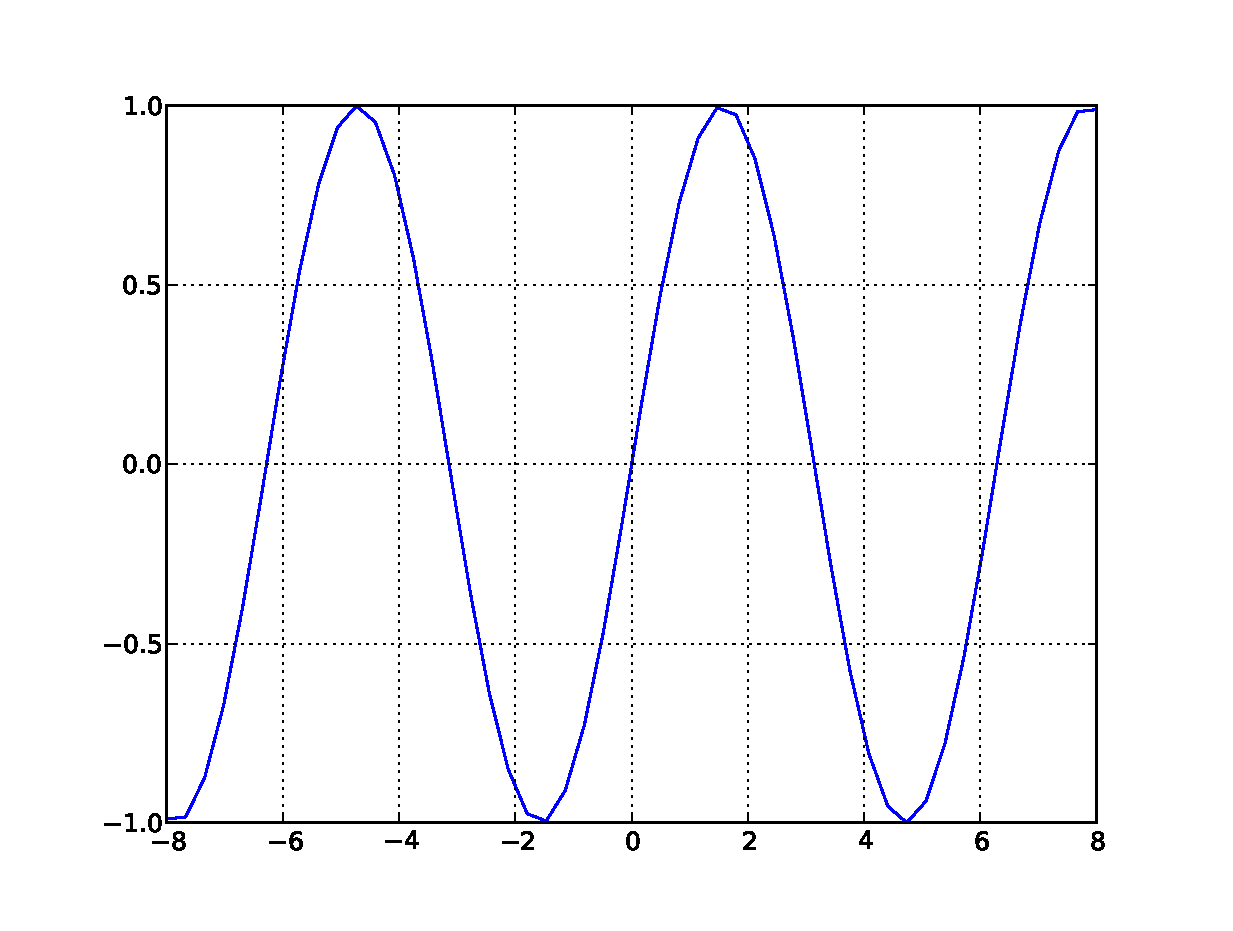
\includegraphics[scale=0.4]{raices00.eps} 
\end{figure}
\end{frame}
\begin{frame}
Las raíces de un polinomio pueden ser reales o complejas.
\\
\bigskip
Si un polinomio tiene coeficientes reales
\[ a_{0},a_{1},a_{2},\ldots,a_{n-1},a_{n} \]
entonces todas las raíces complejas siempre ocurrirán en pares conjugados complejos.
\end{frame}
\begin{frame}
Por ejemplo, un polinomio cúbico tiene la siguiente
forma general:
\[ f(x)= a_{0}x^{3}+a_{1}x^{2}+a_{2}x+a_{3}\]
\begin{enumerate}
\item Tres raíces reales distintas.
\item Una raíz real con multiplicidad 3.
\item Una raíz real simple y una raíz real con multiplicidad 2.
\item Una raíz real y un par conjugado complejo.
\end{enumerate}
\end{frame}
\begin{frame}[fragile]
\frametitle{Tres raíces distintas}
\begin{minipage}{5cm}
\fontsize{12}{12}\selectfont
\[ \begin{split}
f(x)=& x^{3} - 3x^{2}-x+3 \\
=& (x-3)(x+1)(x-1)
\end{split} \]
Las raíces son:
\[ \begin{split}
x_{1} =& 3 \\
x_{2} =& -1 \\
x_{3} =& 1 \\
\end{split}\]
\end{minipage}
\hspace{0.5cm}
\begin{minipage}{4.5cm}
\begin{figure}
	\centering
	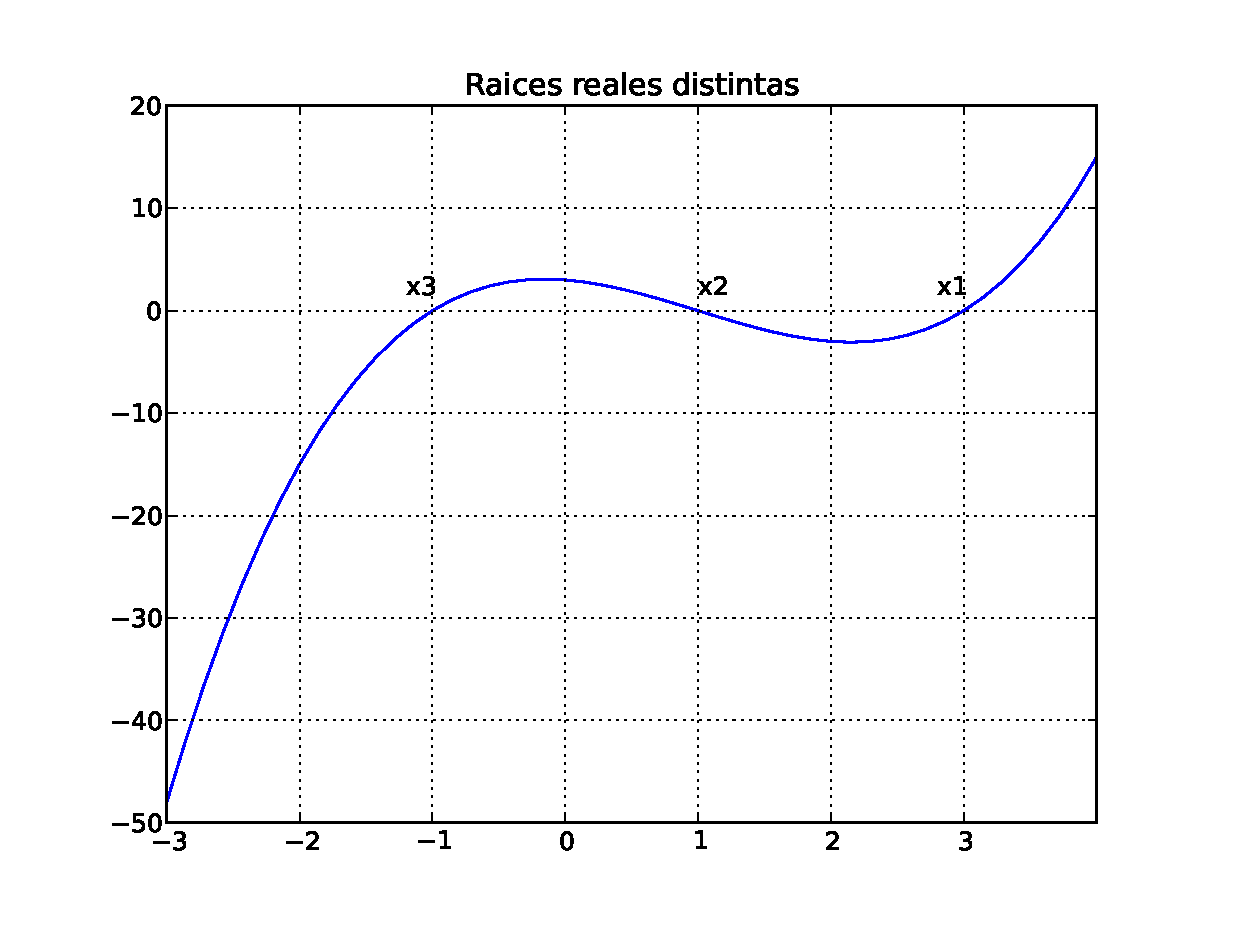
\includegraphics[scale=0.3]{raices01.eps} 
\end{figure}
\end{minipage}
\end{frame}
\begin{frame}[fragile]
\frametitle{Raíz real con multiplicidad 3}
\begin{minipage}{5cm}
\fontsize{12}{12}\selectfont
\[ \begin{split}
f(x)=& x^{3} - 6x^{2} + 12x - 8 \\
=& (x-2)^{3}
\end{split} \]
Las raíces son:
\[ \begin{split}
x_{1} =& 2 \\
x_{2} =& 2 \\
x_{3} =& 2 \\
\end{split}\]
\end{minipage}
\hspace{0.5cm}
\begin{minipage}{4.5cm}
\begin{figure}
	\centering
	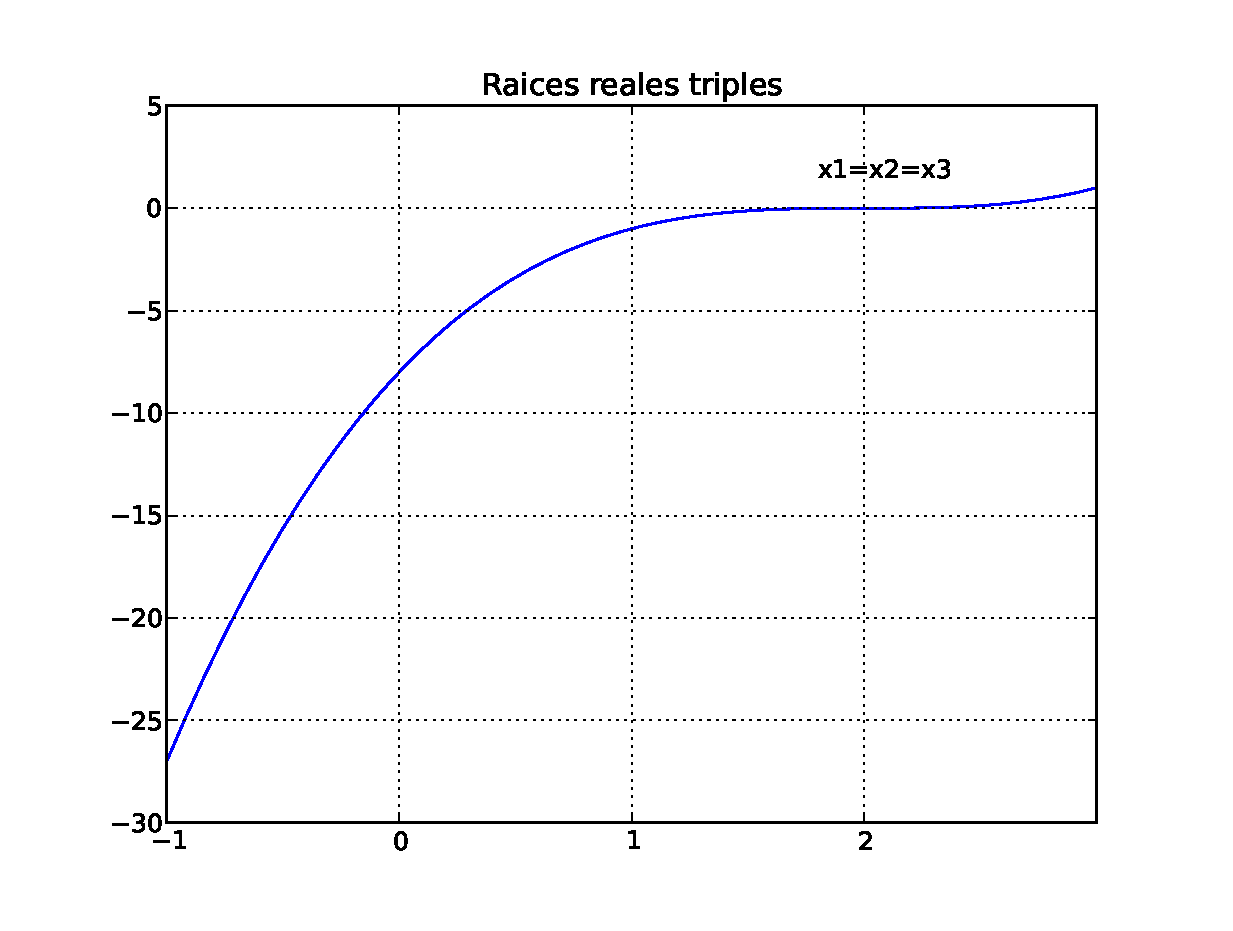
\includegraphics[scale=0.3]{raices02.eps} 
\end{figure}
\end{minipage}
\end{frame}
\begin{frame}[fragile]
\frametitle{Raíz real simple y \\ una raíz real con multiplicidad 2}
\begin{minipage}{5cm}
\fontsize{12}{12}\selectfont
\[ \begin{split}
f(x)=& x^{3} - 12x + 16 \\
=& (x+4)(x-2)^{2}
\end{split} \]
Las raíces son:
\[ \begin{split}
x_{1} =& -4 \\
x_{2} =& 2 \\
x_{3} =& 2 \\
\end{split}\]
\end{minipage}
\hspace{0.5cm}
\begin{minipage}{4.5cm}
\begin{figure}
	\centering
	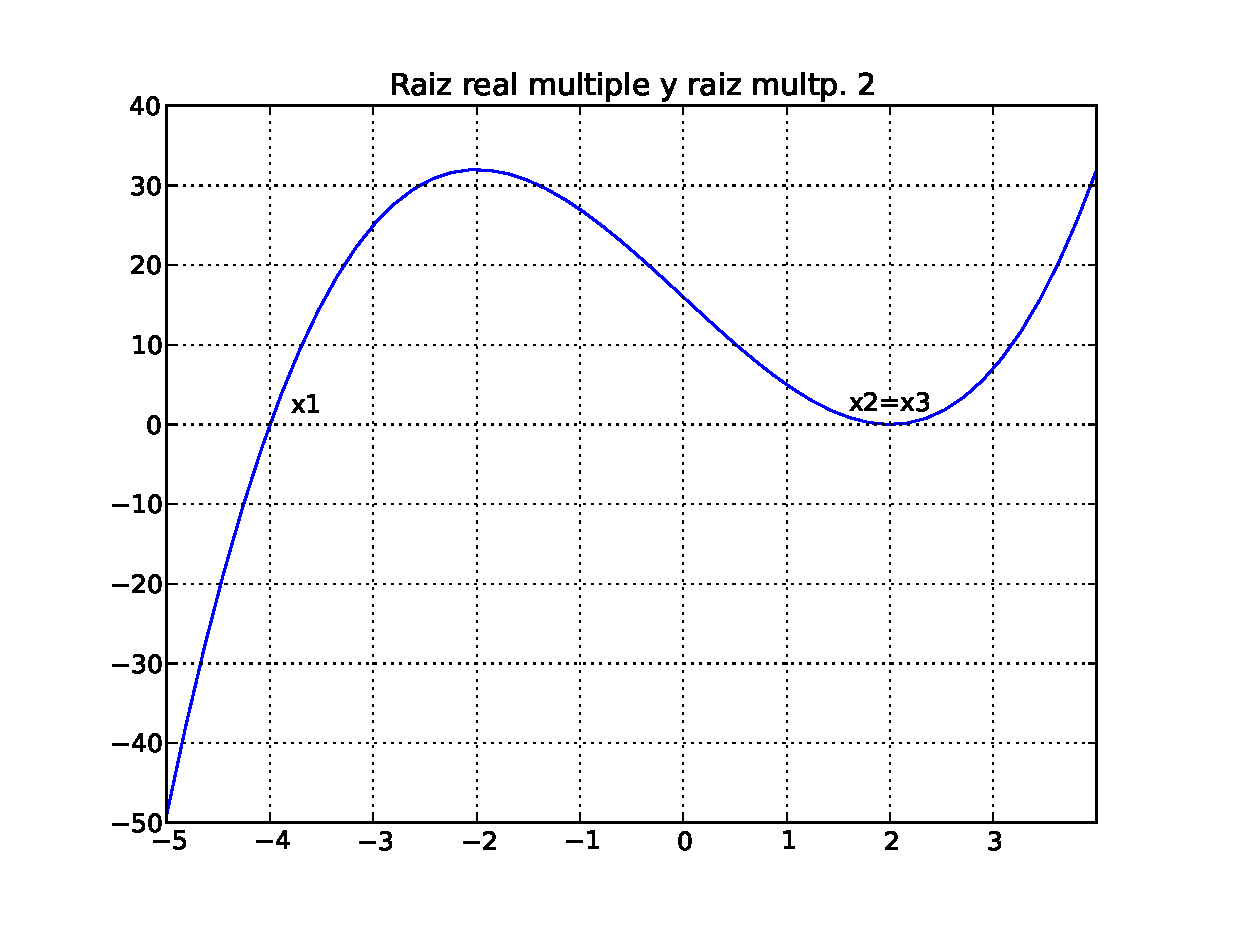
\includegraphics[scale=0.3]{raices03.eps} 
\end{figure}
\end{minipage}
\end{frame}
\begin{frame}[fragile]
\frametitle{Raíz real y un par conjugado complejo}
\begin{minipage}{5cm}
\fontsize{12}{12}\selectfont
\[ \begin{split}
f(x)=& x^{3} - 2x^{2}- 3x +10  \\
=& (x+2)(x- (2+i))* {}\\
*& (x-(2-i))
\end{split} \]
Las raíces son:
\[ \begin{split}
x_{1} =& -2 \\
x_{2} =& 2+i \\
x_{3} =& 2-i \\
\end{split}\]
\end{minipage}
\hspace{0.5cm}
\begin{minipage}{4.5cm}
\begin{figure}
	\centering
	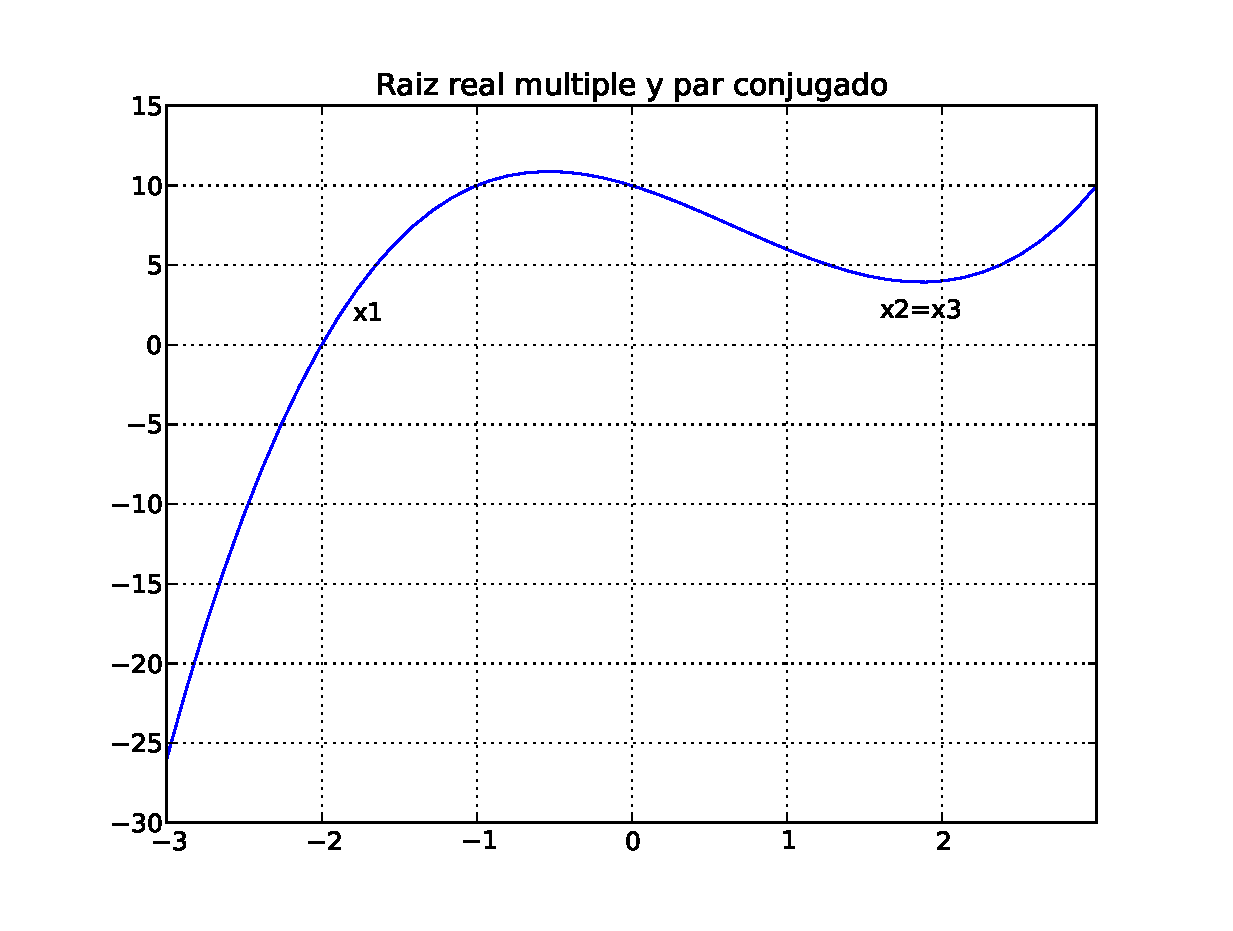
\includegraphics[scale=0.3]{raices04.eps} 
\end{figure}
\end{minipage}
\end{frame}
\section{Funciones algebraicas}
\begin{frame}
\frametitle{Funciones algebraicas}
Sea $g=f(x)$ la función expresada como
\[ f_{n}y^{n} + f_{n-1}y^{n-1} + \ldots + f_{1}y + f_{0} = 0 \]
Donde $f_{i}$ es un polinomio de orden $i$ en $x$.
\\
\bigskip
Los polinomios son un caso simple de funciones algebraicas que se representan generalmente como
\[f_{n}(x) = a_{0} + a_{1}x + a_{2} x^{2}+ \ldots +a_{n}x^{n} \]
Donde $n$ es el orden del polinomio.
\end{frame}
\section{Funciones trascendentales}
\begin{frame}
\frametitle{Funciones trascedentales}
Son aquellas que no son algebraicas.
\\
\bigskip
Comprenden a las funciones trigonométricas, exponenciales, logarítmicas, entre otras.
\\
\bigskip
Ejemplos:
\begin{itemize}
\item \[ f(x)=ln(x^{2}-1) \]
\item \[g(x)=e^{-0.2x} \sin(3x-5) \]
\end{itemize}
\end{frame}
\begin{frame}
Los métodos numéricos estándar para encontrar raíces pueden clasificarse en dos rubros:
\\
\bigskip
\textbf{1.} La determinación de las raíces reales de ecuaciones algebraicas y trascendentales. Las técnicas a emplear en estos casos se diseñaron con el fin de encontrar el valor de una raíz simple de acuerdo con un conocimiento previo de su posición aproximada.
\end{frame}
\begin{frame}
\textbf{2.} La determinación de todas las raíces reales y complejas de un polinomio, para lo cual los métodos numéricos estén diseñados específicamente para polinomios. 
\\
\bigskip
Determinan sistemáticamente todas las raíces del polinomio en lugar de hacerlo sólo con una, dada la posición aproximada.
\end{frame}
\section{Método de incrementos sucesivos}
\begin{frame}
\frametitle{Método de incrementos sucesivos}
Podemos aproximar mucho mejor las raíces de una función, cuando la graficamos.
\\
\bigskip
Con una gráfica general de unos cuantos puntos, tendríamos lo necesario para considerar los valores de las raíces.
\\
\bigskip
El método de búsqueda incremental es una herramienta útil que podemos adoptar en conjunto con otras estrategias de cálculo de raíces, por sí sólo, éste método no nos ofrece más que una referencia sobre en dónde podrían estar esas raíces.
\end{frame}
\begin{frame}
La idea básica detrás del método de búsqueda incremental es simple: si $f(x_{1})$ y $f(x_{2})$ tienen signos opuestos, entonces hay al menos una raíz en el intervalo $(x_{1}, x_{2})$.
\end{frame}
\begin{frame}[fragile]
\frametitle{Caso en donde es posible encontrar la raíz}
\begin{center}
	\begin{tikzpicture}[font=\footnotesize, scale=1.3]
		\draw[<->](0,0) -- (6,0);
		\draw[<->](3,-2) -- (3,2);
		\draw [red] (0.5,1.5) .. controls (2,0.2) and (4,-1) .. (5.5,-1.5);
		\draw[dashed] (1,0) -- (1,1.1);
		\draw (0.9,-0.2) node {a}; 
		\draw (1.2,1.4) node {f(a)};
		\draw[dashed] (5,0) -- (5,-1.33);
		\draw (5,0.2) node {b}; 
		\draw (5,-1.7) node {f(b)};
		\draw(4.5,1.5) node {$f(a)*f(b)<0$};
	\end{tikzpicture}
\end{center}
\end{frame}
\begin{frame}
\frametitle{Caso en donde no es posible encontrar la raíz}
\begin{center}
	\begin{tikzpicture}[font=\footnotesize, scale=1.3]
		\draw[<->](0,0) -- (6,0);
		\draw[<->](3,-1) -- (3,3);
		\draw [red] (0.5,2.5) .. controls (2.5,0.5) and (3.5,0.5) .. (5.5,2.5);
		\draw [dashed] (1,0) -- (1,2.1);
		\draw (1,-0.2) node {a};
		\draw (1.1,2.2) node {f(a)};
		\draw [dashed] (4.5,0) -- (4.5,1.65);
		\draw (4.5,-0.2) node {b};
		\draw (4.5, 2) node {f(b)};
		\draw (5,3.5) node {$f(a)*f(b)>0$};
	\end{tikzpicture}
\end{center}
\end{frame}
\begin{frame}
Si el intervalo es lo suficientemente pequeño, es probable que contenga una sola raíz. Así, los ceros de $f(x)$ puede ser detectados mediante la evaluación de la función a intervalos $\Delta x$ y mirando cuando se presente un cambio de signo en la función.
\end{frame}
\begin{frame}
Hay varios problemas con el método de búsqueda incremental:
\begin{enumerate}
\item Es posible perder dos raíces muy próximas entre sí, si el incremento de búsqueda $\Delta x$ es mayor que la separación de las raíces.
\item Una raíz doble (dos raíces que coinciden) no será detectada.
\item Algunas singularidades de $f(x)$ se puede confundir con raíces. Por ejemplo, $f(x) = \tan x$. Tiene cambios de signo en $x = \pm 1/2 n\pi$ con $n = 1, 3, 5,\ldots$
\end{enumerate}
\end{frame}
\begin{frame}
Estos puntos no son ceros verdaderos, ya que la función no cruza el eje $x$.
\begin{figure}
	\centering
	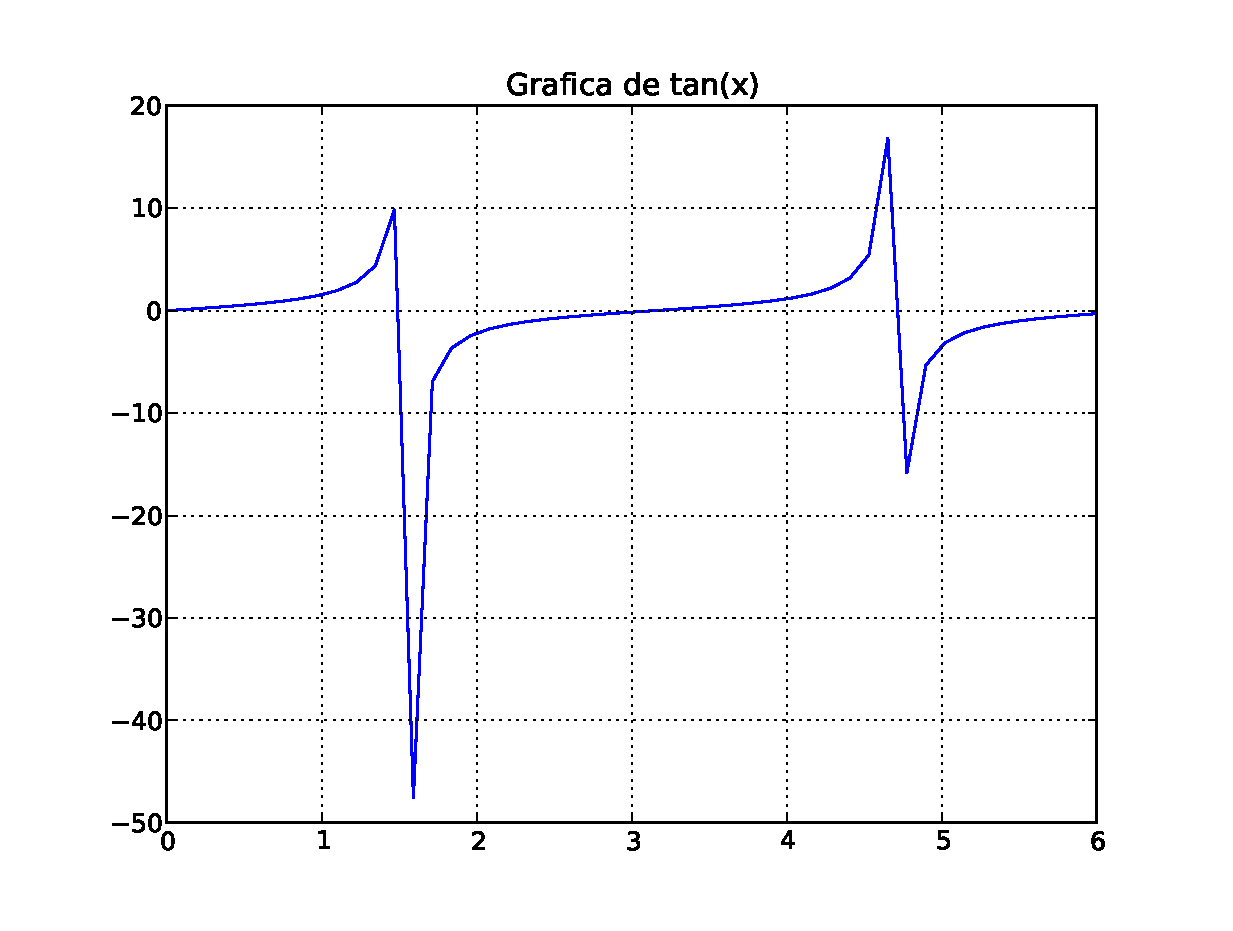
\includegraphics[scale=0.4]{raices05.eps} 
\end{figure}
\end{frame}
\subsection{Código Método de incrementos sucesivos}
\begin{frame}
\frametitle{Código Método de incrementos sucesivos}
El código busca un cero de la función $f$ que proporciona el usuario en el intervalo
$(a,b)$ en incrementos de $dx$.
\\
\bigskip
Se devuelve el intervalo $(x_{1}, x_{2})$ donde se encuentra la raíz, si la búsqueda
se ha realizado correctamente; se devuelve $x_{1} = x_{2} = \mathsf{None}$ cuando no se encontraron raíces.
\\
\bigskip
Luego de que se encontró la primera raíz, (la más cercana al punto $a$), se puede llamar de nuevo al procedimiento, sustitiyendo $x_{2}$ con el fin de encontrar la siguiente raíz. Esto se puede repetir siempre y cuando se detecta una raíz.
\end{frame}
\begin{frame}[fragile]
\begin{lstlisting}
def buscaraiz(f,a,b,dx):
    x1 = a; f1 = f(a)
    x2 = a + dx; f2 = f(x2)
    while f1*f2 > 0.0:
        if x1 >= b: return None
        x1 = x2; f1 = f2
        x2 = x1 + dx; f2 = f(x2)
    else:
        return x1,x2
\end{lstlisting}
\end{frame}
\begin{frame}
\frametitle{Ejemplo}
Usa el método de incrementos sucesivos y con $\Delta x= 0.2$, para estimar la raíz con el valor positivo más pequeño de la función:
\[ f(x) = x^{3} - 10 x^{2} + 5\]
\end{frame}
\begin{frame}
\begin{figure}
	\centering
	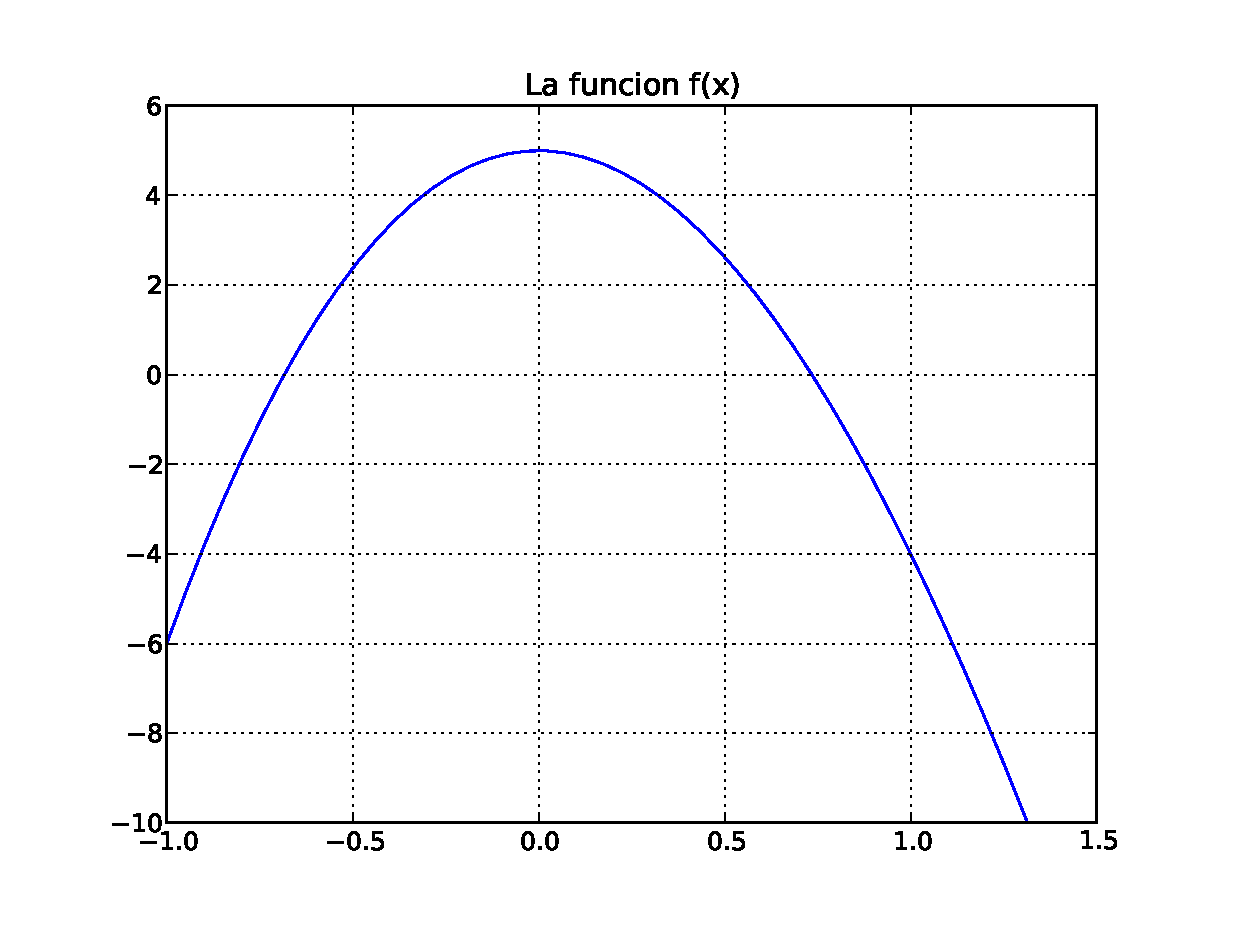
\includegraphics[scale=0.5]{raices06.eps} 
\end{figure}
\end{frame}
\begin{frame}[fragile]
\begin{lstlisting}
def f(x): return x**3 - 10*x**2 + 5.

a, b, dx = (0.0,1.5, 0.2)

print 'El intervalo es: '
x1, x2 = buscaraiz(f,a,b,dx)
print x1,x2
\end{lstlisting}
\end{frame}
\section{Método de Bisección}
\begin{frame}
\frametitle{{Método de Bisección}}
Después de que se ha identificado una raíz $f(x) = 0$ en el intervalo $(x_{1}, x_{2})$, disponemos de varios métodos para encontrar el valor de la raíz.
\\
\bigskip
El método de bisección logra esta tarea: \textcolor{red}{el intervalo se reduce sucesivamente a la mitad  hasta que se vuelve suficientemente pequeño}. La técnica de bisección no es el método más rápido disponible, pero es el más fiable. Una vez que una raíz se ha encontrado en un intervalo, nos podemos acercar a ella.
\end{frame}
\begin{frame}
El método de bisección utiliza el mismo principio que el incremento sucesivo: si hay una raíz en el intervalo $(x_{1}, x_{2})$, entonces $f(x_{1})*f(x_{2})<0$.
\end{frame}
\begin{frame}
Con el fin de reducir a la mitad el intervalo, se calcula $f(x_{3})$, donde $x_{3} = (x1 + x2)/2$ es el punto medio del intervalo.
\end{frame}
\begin{frame}
\setbeamercovered{invisible}
\begin{center}
	 \begin{tikzpicture}[font=\footnotesize, scale=1.3]
		\draw[->](0,0) -- (6,0);
		\draw[<->](0,-2) -- (0,2);
		\draw [red] (0.5,1.5) .. controls (2,0.2) and (4,-1) .. (5.5,-1.5);
		\draw[dashed] (1,0) -- (1,1.1);
		\draw (0.9,-0.2) node {$x_{1}$};
		\draw (0.9,1.5) node {$f(x_{1})$}; 
		\draw[dashed] (5,0) -- (5,-1.33);
		\draw (5,0.2) node {$x_{2}$};
		\draw (5,-1.6) node {$f(x_{2})$};\pause
		\draw (3,0.2) node {$x_{3}$};\pause
		\draw [dashed] (3,0) -- (3,-0.3);
		\draw (3,-0.7) node {$f(x_{3})$};
	\end{tikzpicture}
\end{center}
\end{frame}
\begin{frame}
Si $f(x_{1})*f(x_{3}) < 0$, entonces la raíz debe estar en $(x_{1}, x_{3})$ entonces re-emplazamos del intervalo inicial $x_{2}$ por $x_{3}$. De lo contrario, la raíz se encuentra en $(x_{3}, x_{2})$, en tal caso, se sustituye $x_{3}$ por $x_{1}$.
\setbeamercovered{invisible}
\pause
\begin{center}
	 \begin{tikzpicture}[font=\footnotesize]
		\draw[->](0,0) -- (6,0);
		\draw[<->](0,-2) -- (0,2);
		\draw [red] (0.5,1.5) .. controls (2,0.2) and (4,-1) .. (5.5,-1.5);
		\draw[dashed] (1,0) -- (1,1.1);
		\draw (0.9,-0.2) node {$x_{1}$};
		\draw (0.9,1.5) node {$f(x_{1})$}; 
		\draw (3,0.2) node {$x_{2}$};
		\draw [dashed] (3,0) -- (3,-0.3);
		\draw (3,-0.7) node {$f(x_{2})$};\pause
		\draw (2,-0.2) node {$x_{3}$};
		\draw [dashed] (2,0) -- (2,0.3);
		\draw (2,0.7) node {$f(x_{3})$};
	\end{tikzpicture}
\end{center}
\end{frame}
\begin{frame}
En cualquiera de los casos, el nuevo intervalo $(x_{1}, x_{2})$ es la mitad del tamaño del intervalo original. La bisección es repite hasta que el intervalo se ha reducido a un valor $\epsilon$ pequeño, de modo que
\[ \vert x_{2} - x_{1} \vert \leq \epsilon\]
\end{frame}
\begin{frame}
Es fácil calcular el número de bisecciones necesarias para alcanzar el valor de $\epsilon$. El intervalo inicial $\Delta x$, se reduce a $\Delta x /2$ en la primera bisección, $\Delta x /2^{2}$ en la segunda, luego de $n$ bisecciones, $\Delta x /2^{n}$. Haciendo $\Delta x /2^{n} = \epsilon$, resolvemos para $n$
\[ n = \dfrac{ln(\vert \Delta x \vert/ \epsilon)}{ln 2}\]
\end{frame}
\begin{frame}[fragile]
\frametitle{Algoritmo para el método de bisección}
	\begin{lstlisting}
	def bisect(f,x1,x2,switch,epsilon=1.0e-9):
    f1 = f(x1)
    if f1 == 0.0: return x1
    f2 = f(x2)
    if f2 == 0.0: return x2
    
    if f1*f2 > 0.0: print 'La raiz no se ha identificado en un intervalo'

    n = ceil(log(abs(x2 - x1)/epsilon)/log(2.0))
	\end{lstlisting}
\end{frame}
\begin{frame}[fragile]
La función \texttt{ceil} devuelve el menor entero mayor o igual a $x$.
\\
\medskip
Ejemplos:\\
\medskip
\verb|>>>ceil(1.1) # 2.0| \\
\verb|>>>ceil(1.6) # 2.0| \\
\verb|>>>ceil(-1.1) # -1.0| \\
\verb|>>>ceil(-1.6) # -1.0|
\end{frame}
\begin{frame}[fragile]
\frametitle{Algoritmo para el método de bisección}
	\begin{lstlisting}
    for i in np.arange(n):
        x3 = 0.5*(x1 + x2); f3 = f(x3)
        if (switch == 0) and (abs(f3) > abs(f1)) \
                        and (abs(f3) > abs(f2)):
            return None
        if f3 == 0.0: return x3
        if f2*f3 < 0.0:
            x1 = x3; f1 = f3
        else:
            x2 =x3; f2 = f3
    return (x1 + x2)/2.0
	\end{lstlisting}

\end{frame}
\begin{frame}
Haciendo que la variable \texttt{switch} = 1, se forza la rutina para comprobar si la magnitud de $f(x)$ disminuye con la reducción a la mitad de cada intervalo.
\\
\medskip
Si no es así, algo anda mal (probablemente la ''raíz" no es una raíz en absoluto, sino una singularidad) y se devuelve la \texttt{raíz} = \texttt{None}. Dado que esta característica no siempre es deseable, el valor predeterminado es \texttt{switch}=0.
\end{frame}
\begin{frame}
Veamos lo que hace la variable \texttt{switch}:
\\
\medskip
Hasta el momento no nos hemos fijado en la magnitud de $f(x_{1})$ y $f(x_{2})$, sólo y en el signo del respectivo producto, pero ahora, tomamos en cuenta la magnitud tanto de los puntos evaluados en la función como del producto mismo.
\\
\medskip
Consideremos le primer caso de la función $f(x)$, donde ya sabemos que hay una raíz en el intervalo $[0.6,0.8]$
\end{frame}
\begin{frame}[fragile]
\frametitle{El valor por defecto de \texttt{switch} = 0}
\begin{tabular}{l | l | l | l | c}
$x_{1}$ & $x_{2}$ & $f(x_{1})$ & $f(x_{2})$ & $f(x_{1})f(x_{2})$ \\ \hline
0.0 & 0.2 & 5.0 & 4.608 & 23.04 \\ \hline
0.2 & 0.4 & 4.608 & 3.464 & 15.9621 \\ \hline
0.4 & 0.6 & 3.464 & 1.616 & 5.5978 \\ \hline
0.6 & 0.8 & 1.616 & -0.888 & -1.4350 \\ \hline
0.8 & 1.0 & -0.888 & -4.0 & 3.552 \\ \hline
1.0 & 1.2 & -4.0 & -7.672 & 30.688
\end{tabular}
%\begin{tikzpicture}[overlay]
% Define the circle paths
%	\draw [blue](1.north west) -- (1.north east) -- (2.south east) -- (2.south west) -- cycle;
%	\draw [red](3.north west) -- (3.north east) -- (4.south east) -- (4.south west) -- cycle;
%\end{tikzpicture}
\end{frame}
\begin{frame}[fragile]
Del código tenemos que:
\begin{verbatim}
if (switch == 0) and (abs(f3) > abs(f1)) \ 
                 and (abs(f3) > abs(f2)):
    return None
\end{verbatim}
\begin{tabular}{l  l | l | l}
$abs(f3) > abs(f1)$ & $abs(f3) > abs(f2)$ & Expresión \\ \hline
\texttt{True} & \texttt{True} & True \\ \hline

\end{tabular}
Aquí tendrán que completar la tabla de tal manera que revisen el resultado de la expresión compuesta.
\end{frame}
\begin{frame}
\frametitle{Ejercicios}
Implementa el método de bisección para calcular el(los) intervalo(s) y la(s) raíz(ces) de:
\begin{eqnarray*}
	f(x) &=& x^{3} - 10x^{2} + 5 \\
	g(x) &=& x- \tan(x) \hspace{1cm} 0 \leq x \leq 20
\end{eqnarray*}
Con una tolerancia de $1\times 10^{-9}$
\end{frame}
\begin{frame}
Toma en cuenta que $\tan(x)$ es singular y cambia de signo en $x = \pi/2, 3\pi/2,\ldots$. Para no confundir estos puntos para las raíces, hacemos \texttt{switch}= 1.
\\
\medskip
La proximidad de las raíces a las singularidades es otro problema potencial que puede ser prevenido mediante el uso de $\Delta x$ pequeña, usa $x = 0.01$.
\end{frame}
\begin{frame}
\frametitle{Graficas de las funciones y sus raíces}
\begin{figure}
	\centering
	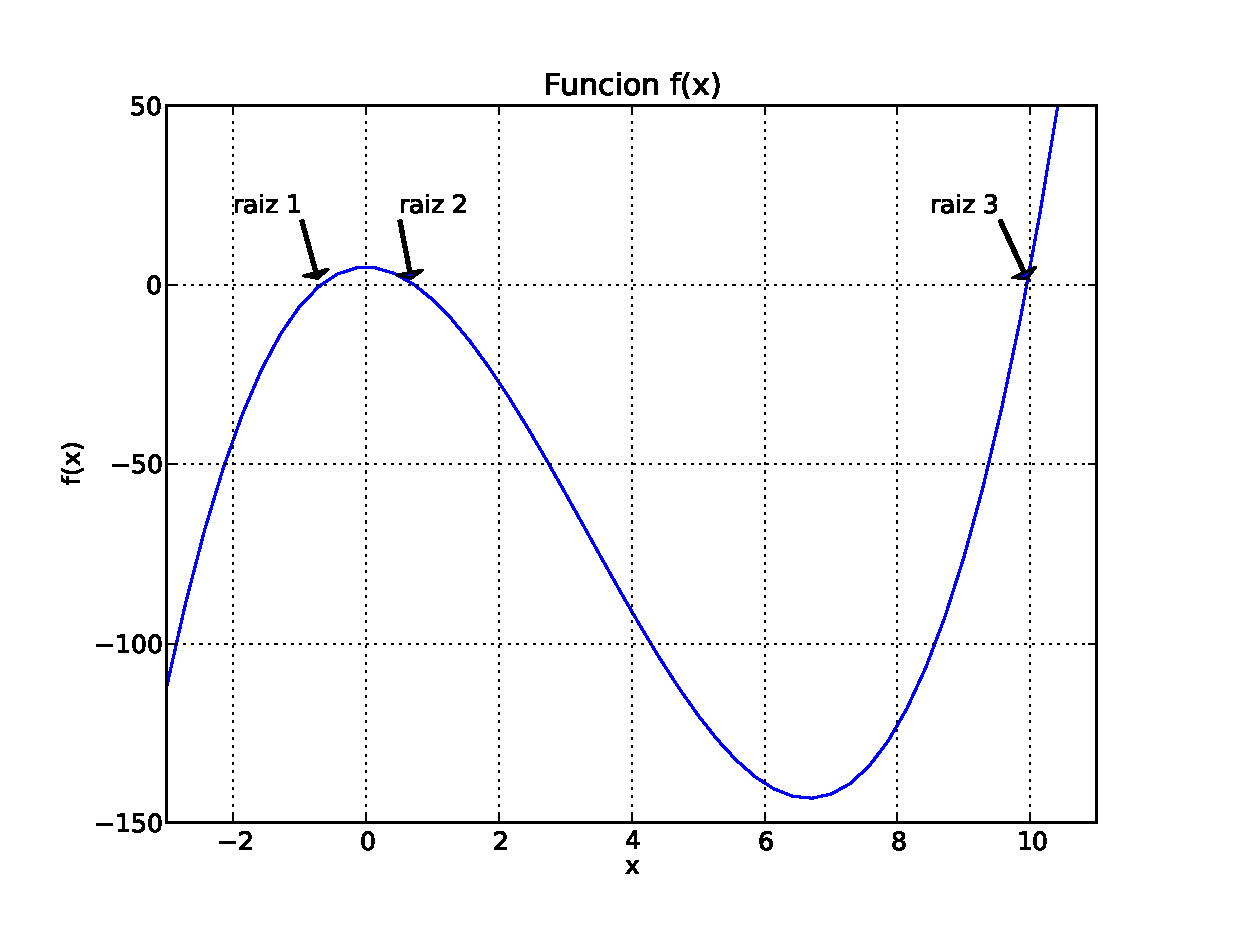
\includegraphics[scale=0.4]{ejercicio1_Biseccion.eps}<1>
	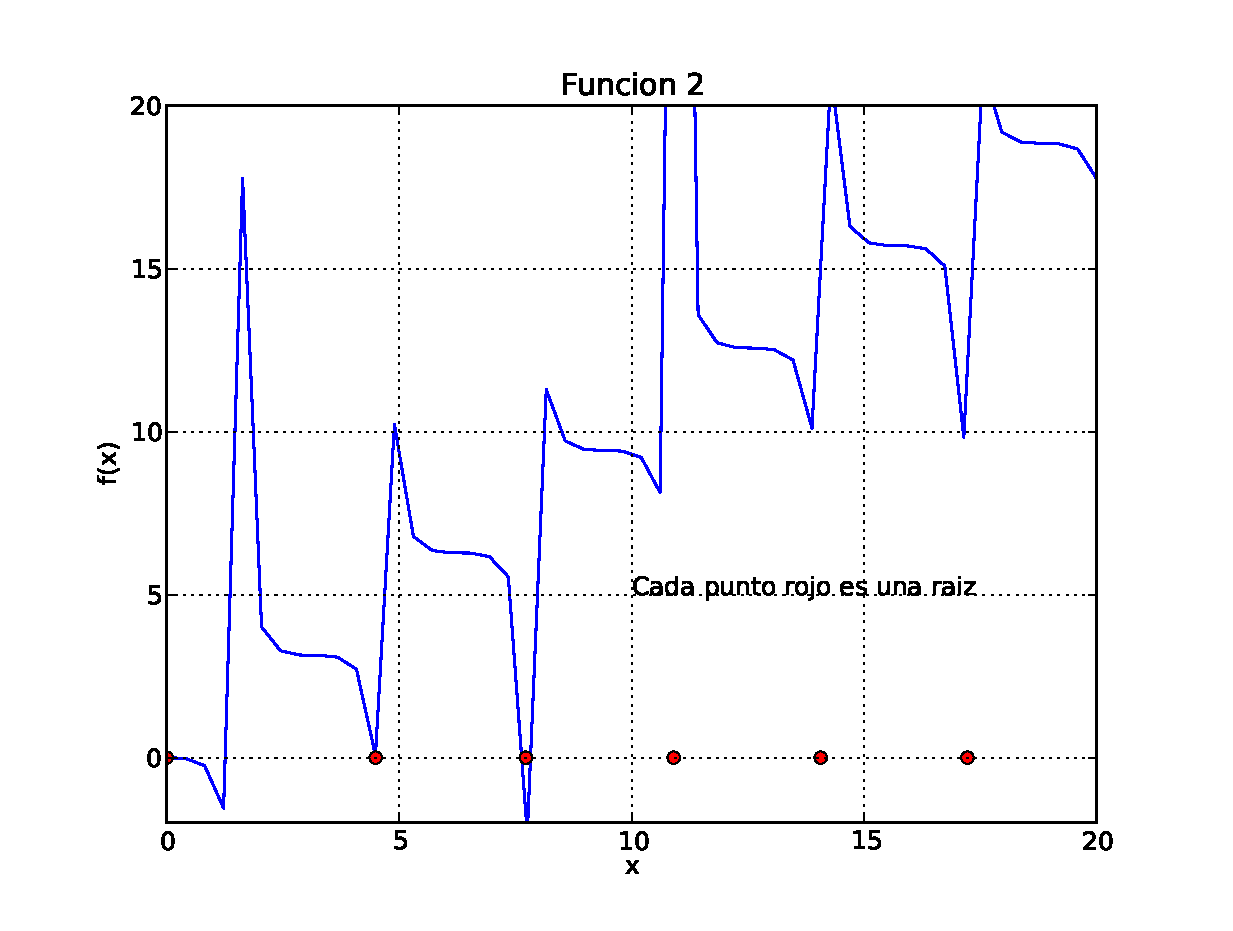
\includegraphics[scale=0.4]{ejercicio2_Biseccion.eps}<2>
\end{figure}
\end{frame}
\begin{frame}
\frametitle{Estrategia de solución}
Para integrar los elementos que hemos visto:
\begin{enumerate}
\item Recuperamos el algoritmo que nos identifica en qué intervalo se encuentra una raíz.
\item Aplicamos el algoritmo del método de bisección.
\item Usamos un ciclo que nos revise en el dominio que se nos proporciona, si existe más de una raíz.
\end{enumerate}
\end{frame}
\begin{frame}[fragile]
\begin{lstlisting}
def f(x): return x**3-10*x**2+5

a,b,dx = (-2.0,11.0,0.02)
	
print 'Intervalo (x1,x2)   raiz'
while 1:
    try:
        x1, x2 = buscaraiz(f,a,b,dx)
    except Exception, e:
        print e; break
    if x1 != None:
        a = x2
        root = bisect(f,x1,x2,0)
        if raiz != None: print '(%2.4f, %2.4f) %2.8f' %(x1, x2, raiz)
\end{lstlisting}
\end{frame}
\begin{frame}[fragile]
\begin{lstlisting}
    else:
        print '\nHecho'
        break
\end{lstlisting}
\end{frame}
\section{Método de Newton-Raphson}
\begin{frame}
\frametitle{Método de Newton-Raphson}
El método de Newton-Raphson es el algoritmo más conocido para encontrar raíces por una buena razón: es simple y rápido.
\\
\medskip
El único detalle es que utiliza la derivada $f'(x)$ así como la función $f(x)$. Por tanto, en los problemas a resolver con este algoritmo, deberá de contemplarse que la derivada sea fácil de calcularse.
\end{frame}
\begin{frame}
El método de N-R se obtiene de la expansión en series de Taylor de $f(x)$ alrededor de $x$:
\[ f(x_{i+1})  = f(x_{i})+ f'(x_{i})(x_{i+1}-x_{i}) + O(x_{i+1}-x_{i})^{2}\]
\end{frame}
\begin{frame}
Si $x_{i+1}$ es una raíz de $f(x)=0$, tenemos que:
\[ 0 = f(x_{i}) + f'(x_{i})(x_{i+1}-x_{i})+ O(x_{i+1}-x_{i})^{2} \]
Suponiendo que $x_{i}$ está cerca de $x_{i+1}$, podemos eliminar el último término de la ecuación y resolver para $x_{i+1}$, por lo que la fórmula de Newton-Raphson es:
\[ x_{i+1} = x_{i} - \dfrac{f(x_{i})}{f'(x_{i})} \]
\end{frame}
\begin{frame}
Si $x$ representa el valor verdadero de la raíz, el error en $x_{i}$ es $E_{i}=x-x_{i}$. Se puede demostrar que si $x_{i+1}$ se calcula de la expresión de N-R, el error es:
\[ E_{i+1} = - \dfrac{f''(x_{i})}{2 f'(x_{i})} E_{i}^{2}\]
Lo que nos dice que el método de N-R converge de manera cuadrática, es decir, el error es el cuadrado del error del punto previo.
\end{frame}
\begin{frame}[fragile]
\frametitle{Representación gráfica}
Podemos interpretar que $x_{i+1}$ es el punto en donde la tangente de $f(x_{i})$ cruza el eje de las $x$:
\begin{center}
	\begin{tikzpicture}[font=\small, scale=0.8]
		\draw [->] (0,0) -- (7,0);
		\draw [<->] (0,-3) -- (0,3);
		\draw [red] (1,3) .. controls (1.5,0.5) and (5,-2) .. (6.5,-2);
		\draw (1,-0.3) node {$x_{i}$};
		\draw (1,3.3) node {$f(x_{i})$};
		\draw [dashed] (1.2,0) -- (1.2,2.35);
		\draw (0.8,3.1) -- (2.35,-0.1);
		\draw [dashed] (2.3,0) -- (2.3,0.58);
		\draw (2.3,-0.3) node {$x_{i+1}$};
	\end{tikzpicture}
\end{center}
\end{frame}
\begin{frame}
El método de N-R es sencillo: se aplica la expresión para $x_{i+1}$ iniciando con un valor $x_{0}$, hasta alcanzar un criterio de convergencia:
\[ \vert x_{i+1} - x_{i} \vert < \epsilon \]
El algoritmo es el siguiente:
\begin{enumerate}
\item Sea $x$ un valor inicial para la raíz de $f(x)=0$.
\item Calcular $\Delta x = - f(x)/f'(x)$.
\item Asignar $x \leftarrow x + \Delta x$ y se repiten los pasos 2-3, hasta alcanzar $\vert \Delta x \vert < \epsilon$.
\end{enumerate}
\end{frame}
\begin{frame}[fragile]
Aunque el método de Newton-Raphson converge rápidamente cerca de la raíz, sus características globales de convergencia son pobres. La razón es que la línea tangente no es siempre una aproximación aceptable de la función.
\end{frame}
\begin{frame}[fragile]
\begin{center}
	\begin{tikzpicture}[font=\small, scale=0.8]
		\draw [->] (0,0) -- (4,0);
		\draw [<->] (0,-1) -- (0,3);
		\draw [red] (1,3) .. controls (2,3) and (2.5,2) .. (3.5,-2);
		\draw (1.2,3) circle (0.05);
		\draw [blue, ->] (1.2,3) -- (3.5,2.7);
		\draw (4.2,0) node {$x$};
		\draw (-0.5,2) node {$f(x)$};
		\draw [dashed] (1.2,0) -- (1.2,3);
		\draw (1.2,-0.2) node {$x_{0}$};
	\end{tikzpicture}
\end{center}
\end{frame}
\begin{frame}[fragile]
\begin{center}
\setbeamercovered{invisible}
	\begin{tikzpicture}[decoration={
  markings,% activar las marcas
  mark= at position 2cm with{\arrow{stealth}}}]
		\draw [->] (0,0) -- (6,0);
		\draw [<->] (0,-2) -- (0,2);
		\draw [red] (0.5,-2) .. controls (3,-1.9) and (3,1.9) .. (5.5,2);
		\draw (4.5,-0.3) node {$x_{0}$};\pause
		\draw [dashed] (4.5,0) -- (4.5,1.69);
		\draw (4.5,1.7) circle (0.04);
		\draw [blue, postaction={decorate}] (4.5,1.7) -- (1,0);
		\draw (1,0.3) node {$x_{1}$};
		\draw (1,0) circle (0.04);\pause
		\draw [dashed] (1,0) -- (1,-1.95);
		\draw (1,-1.95) circle (0.04);
		\draw [blue,, postaction={decorate}] (1,-1.95) -- (5.8,0.1);
	\end{tikzpicture}
\end{center}
\end{frame}
\subsection{Algoritmo para el método Newton-Raphson}
\begin{frame}
\frametitle{Algoritmo para el método Newton-Raphson}
La siguiente algoritmo para el método de Newton-Raphson supone que la raíz a calcularse inicialmente está en el intervalo (a, b).
\\
\medskip
El punto medio del intervalo se utiliza como aproximación inicial de la raíz. Los extremos del intervalo se actualizan luego de cada iteración. Si una iteración del método Newton-Raphson no se mantiene dentro del intervalo, se descarta y se reemplaza
con el método de bisección.
\\
\medskip
Ya que el método \texttt{newtonRaphson} utiliza la función $f(x)$, así como su derivada, (denotadas por $f$ y $df$) deben ser proporcionadas por
el usuario.
\end{frame}
\begin{frame}[fragile]
\frametitle{Algoritmo de \texttt{Newton-Raphson}}
\begin{lstlisting}
def newtonRaphson(f,df,a,b,tol=1.0e-9):
    fa = (f(a)
    if fa == 0.0: return a
    fb = f(b)
    if f(b) == 0.0: return b
    if fa*fb > 0.0: print 'La raiz no esta en el intervalo'
    x = 0.5 * (a + b)
\end{lstlisting}
\end{frame}
\begin{frame}[fragile]
\begin{lstlisting}
    for i in range(30):
        fx = f(x)
        if abs(fx) < tol: return x

        if fa*fx < 0.0:
            b = x
        else:
            a = x; fa = fx
\end{lstlisting}
\end{frame}
\begin{frame}[fragile]
\begin{lstlisting}
        dfx = df(x)
        
        try: dx = -fx/dfx
        except ZeroDivisionError: dx = b - a
        x =  x + dx
        
        if(b - x)*(x - a) < 0.0:
            dx = 0.5*(b-a)
            x = a + dx
        
        if abs(dx) < tol*max(abs(b),1.0): return x
    
    print 'Son demasiadas iteraciones'
\end{lstlisting}
\end{frame}
\begin{frame}
\frametitle{Ejercicio}
Encontrar la raíz positiva más pequeña de
\[ f(x) = x^{4} - 6.4 x^{3} + 6.45x^{2} + 20.538x - 31.752\]
\begin{figure}
	\centering
	\visible<2-> {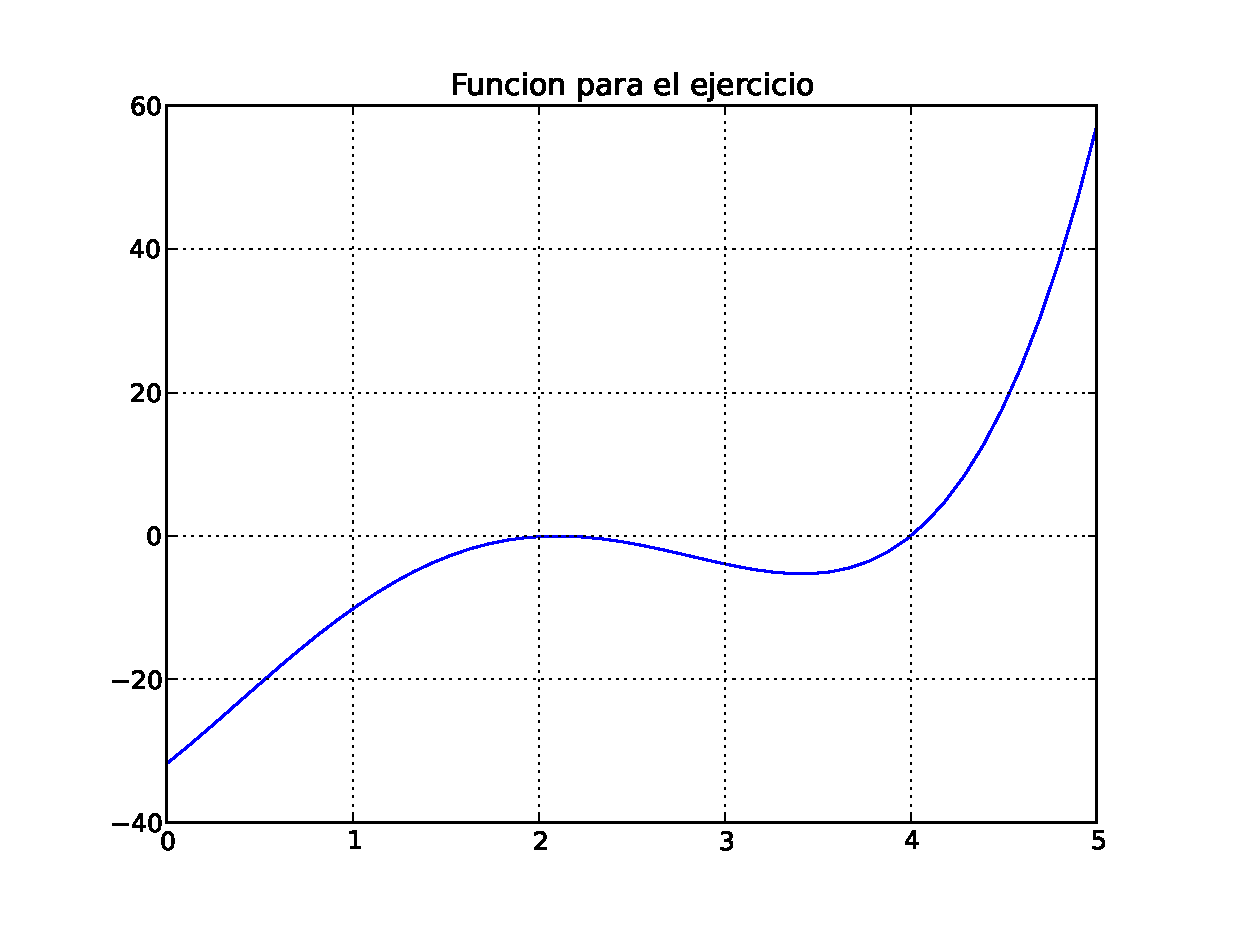
\includegraphics[scale=0.3]{raices08.eps}}
\end{figure}
\end{frame}
\begin{frame}[fragile]
\begin{lstlisting}
def f(x): return x**4 - 6.4*x**3 + 6.45*x**2 + 20.538*x - 31.752
def df(x): return 4.0*x**3 - 19.2*x**2 + 12.9*x + 20.538

def newtonRaphson(x,tol=1e-05):
    for i in range(30):
        dx = -f(x)/df(x)
        x = x + dx
        if abs(dx) < tol: return x,i
    print 'Son demasiadas iteraciones\n'

raiz,numIter = newtonRaphson(2.0)

print 'Raiz =',raiz
print 'Numero de iteraciones =',numIter
\end{lstlisting}
\end{frame}
\begin{frame}
\frametitle{Ejercicios}
\begin{enumerate}
\item Encuentra las raíces de $x \sin x + 3 \cos x - x = 0$ en el intervalo $(-6,6)$ \\
\item Calcula todas las raíces reales de $x^{4} + 0.9x^{3} - 2.3x^{2} + 3.6x - 25.2 = 0$. \\
\item Calcula todas las raíces reales de $x^{4} + 2x^{3} - 7x^{2} + 3 = 0$. \\
\item Calcula todas las raíces de $\sin x - 0.1x = 0$.
\end{enumerate}
\end{frame}
\section{Método de la falsa posición}
\begin{frame}
\frametitle{Método de la falsa posición}
Este método es parecido al de bisección, ya que el intervalo que contiene a la raíz se va reduciendo.
\\
\bigskip
En vez de bisectar de manera monótona el intervalo, se utiliza una interpolación lineal ajustada a dos puntos extremos para encontrar la aproximación de la raíz.
\end{frame}
\begin{frame}
La función está bien aproximada por la interpolación lineal, con lo que las raíces tendrán una buena precisión; la iteración convergerá más rápido que como ocurre con el método de bisección.
\end{frame}
\begin{frame}
Dado un intervalo $[a,c]$ que contenga a la raíz, la función lineal que pasa por $(a,f(a))$ y $(c,f(c))$ se escribe como:
\[ y = f(a) + \dfrac{f(c)-f(a)}{c-a}(x-a) \]
de donde se despeja $x$:
\[ x = a + \dfrac{c-a}{f(c)-f(a)}(y-f(a)) \]
\end{frame}
\begin{frame}
La coordenada $x$ en donde la línea intersecta al eje $x$ se determina al hacer $y=0$ en la ecuación anterior, por tanto:
\[ b = a - \dfrac{c-a}{f(c)-f(a)}f(a) = \dfrac{af(c)-cf(a)}{f(c)-f(a)} \]
\end{frame}
\begin{frame}
Después de encontrar $b$, el intervalo $[a,c]$ se divide en $[a,b]$ y $[b,c]$.
\\
\bigskip
Si $f(a)f(b) \leq 0$, la raíz se encuentra en $[a,b]$; en caso contrario, está en $[b,c]$. Los extremos del nuevo intervalo que contiene a la raíz se renombran para el siguiente paso como $a$ y $c$.
\\
\bigskip
El procedimiento de interpolación se repite hasta que las raíces estimadas convergen.
\end{frame}
\begin{frame}[fragile]
\frametitle{Método de la falsa posición}
\begin{center}
	\begin{tikzpicture}[font=\small]
		\draw [->] (0,0) -- (7,0);
		\draw [<->](0,-3) -- (0,3);
		\draw [red] (1,3) .. controls (1.5,0.5) and (5,-2) .. (6.5,-2);
		\draw (1,-0.3) node {x=a};
		\draw (6,0.3) node {x=c};
		\draw [dashed] (1.2,0) -- (1.2,2.35);
		\draw [dashed] (6.3,0) -- (6.3,-1.98);
		\draw (1.2,2.35) -- (6.3,-1.98);
		\draw  (3,3) node {1a. interpolación};
		\draw [->] (3,2.6) -- (2,2);
		\draw  (5,1) node {1a. aproximación};
		\draw [->] (5,0.6) -- (4.1,0.1);
		\draw [dashed] (4,0) -- (4,-0.9);
	\end{tikzpicture}
\end{center}
\end{frame}
\begin{frame}[fragile]
\frametitle{Método de la falsa posición}
\begin{center}
	\begin{tikzpicture}[font=\small]
		\draw [->] (0,0) -- (7,0);
		\draw [<->] (0,-3) -- (0,3);
		\draw [red] (1,3) .. controls (1.5,0.5) and (5,-2) .. (6.5,-2);
		\draw (1,-0.3) node {x=a};
		\draw (6,0.3) node {x=c};
		\draw [dashed] (1.2,0) -- (1.2,2.35);
		\draw [dashed] (6.3,0) -- (6.3,-1.98);
		\draw (1.2,2.35) -- (6.3,-1.98);
		\draw (1.2,2.35) -- (4,-0.9);
		\draw  (4,2) node {2a. interpolación};
		\draw [->] (4,1.6) -- (2.5,1);
		\draw  (6,1) node {2a. aproximación};
		\draw [->] (5.5,0.8) -- (3.3,0.1);
		\draw [dashed] (4,0) -- (4,-0.9);
		\draw [dashed] (3.25,0) -- (3.25,-0.43); 
	\end{tikzpicture}
\end{center}
\end{frame}
\begin{frame}
La desventaja de este método es que aparecen extremos fijos: uno de los extremos de la sucesión de intervalos no se mueve del punto original, por lo que las aproximaciones a la raíz, denotadas por $b_{1}$, $b_{2}$, $b_{3}$, etc. convergen a la raíz exacta solamente por un lado.
\\
\bigskip
Los extremos fijos no son deseables debido a que hacen más lenta la convergencia, en particular cuando el intervalo es grande o cuando la función
se desvía de manera significativa de una línea recta en el intervalo.
\\
\bigskip
¿Qué podemos hacer al respecto?
\end{frame}
\section{Método de la falsa posición modificado}
\begin{frame}
\frametitle{Método de la falsa posición modificado}
En este método, el valor de $f$ en un punto fijo se divide a la mitad si este punto se ha repetido más de dos veces.
\\
\bigskip
El extremo que se repite se llama extremo fijo. La excepción para esta regla es que para $i=2$, el valor de $f$ en un extremo se divide entre 2 de
inmediato si no se mueve.
\end{frame}
\begin{frame}[fragile]
\frametitle{Método de falsa posición modificado}
\begin{center}
	\begin{tikzpicture}[font=\small]
		\draw [->] (0,0) -- (7,0);
		\draw [<->] (0,-3) -- (0,3);
		\draw [red] (1,3) .. controls (1.5,0.5) and (5,-2) .. (6.5,-2);
		\draw (1,-0.3) node {x=a};
		\draw (6,0.3) node {x=c};
		\draw [dashed] (1.2,0) -- (1.2,2.35);
		\draw [dashed] (6.3,0) -- (6.3,-1.98);
		\draw (1.2,2.35) -- (6.3,-1.98);
		\draw  (3,3) node {1a. interpolación};
		\draw [->] (3,2.6) -- (2,2);
		\draw  (5,1) node {1a. aproximación};
		\draw [->] (5,0.6) -- (4.1,0.1);
		\draw [dashed] (4,0) -- (4,-0.9);
		%\draw [dashed] (1,0) -- (1,2.7); 
	\end{tikzpicture}
\end{center}
\end{frame}
\begin{frame}[fragile]
\frametitle{Método de la falsa posición modificado}
\begin{center}
	\begin{tikzpicture}[font=\small]
		\draw [->] (0,0) -- (7,0);
		\draw [<->] (0,-3) -- (0,3);
		\draw [red] (1,3) .. controls (1.5,0.5) and (5,-2) .. (6.5,-2);
		\draw (1,-0.3) node {x=a};
		\draw (6,0.3) node {x=c};
		\draw [dashed] (1.2,0) -- (1.2,2.35);
		\draw [dashed] (6.3,0) -- (6.3,-1.98);
		\draw (1.2,2.35) -- (6.3,-1.98);
		\draw (1.2,1.3) -- (4,-0.9);
		\draw  (4,2) node {2a. interpolación};
		\draw [->] (4,1.6) -- (1.8,1);
		\draw  (6,1) node {2a. aproximación};
		\draw [->] (5.5,0.8) -- (3.1,0.1);
		\draw [dashed] (4,0) -- (4,-0.9);
	\end{tikzpicture}
\end{center}
\end{frame}
\section{Método de la secante}
\begin{frame}
\frametitle{Método de la secante}
A diferencia del método de Newton, el valor de $f'$ se aproxima utilizando dos valores de iteraciones consecutivas de $f$. Con lo que se elimina la necesidad de evaluar tanto a $f$ como a $f'$ en cada iteración.
\end{frame}
\begin{frame}
Las aproximaciones sucesivas para la raíz en el método de la secante están dadas por:
\[ x_{n} = x_{n-1} - y_{n-1} \dfrac{x_{n-1} - x_{n-2}}{y_{n-1}- y_{n-2}}, \hspace{1cm} n=2,3,\ldots \]
donde $x_{0}$ y $x_{1}$ son dos suposiciones iniciales para comenzar la iteración.
\end{frame}
\begin{frame}[fragile]
\frametitle{Método de la secante}
\setbeamercovered{invisible}
\begin{center}
	\begin{tikzpicture}[font=\small]
		\draw [->] (0,0) -- (7.5,0);
		\draw [->] (0,0) -- (0,4);
		\draw [red](7,3.5) .. controls (6.3,2) and (4.5,0.3) .. (1,0);
		\draw [dashed] (6.8,3.1) -- (6.8,0);
		\draw (6.6,-0.3) node {$x_{0}$};
		\draw (6.6, 3.3) node {$f_{0}$};
		\draw [dashed] (5.5,1.65) -- (5.5,0);
		\draw (5.25,-0.3) node {$x_{1}$};
		\draw (5.25, 1.8) node {$f_{1}$};
		\draw (6.8,3.1) -- (4.1,0);\pause
		\draw (4,-0.3) node {$x_{2}$};
		\draw [dashed] (4.1,0) -- (4.1,0.8);
		\draw (3.9, 1) node {$f_{2}$};\pause
		\draw (5.5,1.65) -- (2.9,0);
		\draw (2.8,-0.3) node {$x_{3}$};
	\end{tikzpicture}
\end{center}
\end{frame}
\begin{frame}
\frametitle{Atento aviso}
En las técnicas de falsa posición, falsa posición modificada y el método de la secante, no hemos presentado como tal un código en \python{} que nos devuelva las raíces, por lo que tendrás que proponer un código para cada una de las técnicas.
\\
\medskip
Ese código lo vas a utilizar par resolver los problmeas y ejercicios del examen.
\end{frame}
\end{document}